\[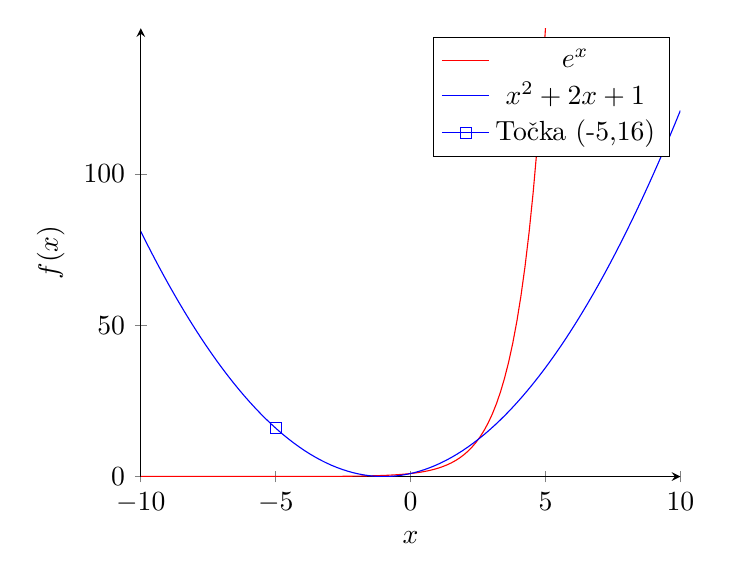
\begin{tikzpicture}

\begin{axis}[axis lines = left,xlabel = \(x\),ylabel = {\(f(x)\)}]%nastavimo parametri kakšen bo sam koordinatni sistem

%Eksponentna funkcija
\addplot [domain=-10:5, samples=100, color=red]{e^x};%domena
\addlegendentry{\(e^x\)} %doda opis funkcij


%Parabola
\addplot [domain=-10:10, samples=100, color=blue]{x^2 + 2*x + 1};
\addlegendentry{\(x^2 + 2x + 1\)}
%dodamo točke na paraboli
\addplot[color=blue, mark=square] coordinates {(-5,16)};\addlegendentry{Točka {(-5,16)}}
    
%Parabola
%\addplot[domain=0:2*pi]{sin(deg(x)}


\end{axis}
\end{tikzpicture}\]